\documentclass[hyperref={pdfpagelabels=false}]{beamer}
\usepackage{graphicx,lmodern,subfigure,ulem,color,graphicx,tikz,booktabs,natbib}
\usepackage{mathrsfs}
\usetheme{Warsaw}
%\definecolor{beamer@blendedblue}{rgb}{0.1,0.5,0.1}
%\definecolor{ForestGreen}{RGB}{60, 140, 60}
%\setbeamercolor{structure}{fg=beamer@blendedblue}
\setbeamertemplate{navigation symbols}{}
\setbeamertemplate{footline}[frame number]
\bibliographystyle{chicago}
\newcommand{\spitem}{\vspace{.3cm}\item}
\newcommand{\elas}{$E_{labor}$}
\def \ourFigPath {../../} 



\title{Noise over the Business Cycle}
\author{Marco Brianti\\Vito Cormun}
\institute{Boston College}
\date{June 2018}


\begin{document}
	
	\frame{
		
		
		\maketitle
}



\frame{\frametitle{Research Question}
	
	The key empirical question is how the effect of \textbf{noise} varies over the \textbf{business cycle}
	
	\
	
	\
	
	We employ a \textbf{regime switching} econometric model where transitions across states (recession and expansion) are \textbf{smooth}
		
}
	

\frame{\frametitle{Econometric Procedure - Overview}
	
	We use a 2-step procedure
	
	\
	
	\begin{enumerate}
		\item Estimate series of noise shocks orthogonal to any other exogenous source of fluctuations
		
		\
		
		\item Estimate a Smooth Transition Local Projection model (hereafter STLP) to estimate dynamic responses of key macroeconomic variables
	\end{enumerate}
	
}


\frame{\frametitle{Step 1 - Overview}
	
	We estimate a noise shock as a change in the expected growth rate of Real GDP which is orthogonal to 
	
	\
	
		\begin{enumerate}
		\item contemporaneous structural shocks
		
		\
		
		\item lagged principal components from a large dataset
		
		\
		
		\item past and future TFP
	\end{enumerate}
	
}


\frame{\frametitle{Step 1 - Estimation of $Z_t$}
	
	Data 
	\begin{itemize}
	 \item $X_t$ is log of Real GDP at time $t$
	 \item $X_{t+k|t} = E[X_{t+k}|I(t)]$ provided by Survey of Professional Forecasters 
	 \end{itemize}
 
 \
 
 Procedure
	$$
	Z_t = (X_{t+4|t} - X_{t|t}) - (X_{t+4|t-1} - X_{t|t-1})
	$$
	where 
	\begin{itemize}
	\item $(X_{t+4|t} - X_{t|t})$ is expected growth rate of Real GDP conditional on information set up to time $t$
	\item $(X_{t+4|t-1} - X_{t|t-1})$ is expected growth rate of Real GDP conditional on information set up to time $t-1$
	\item $Z_t$ is a shock to the expectations of output growth rate
	\end{itemize}
}


\frame{\frametitle{Step 1 - Estimation of $\tilde{Z}_t$}
	\textbf{Problem.} ${Z}_t$ is correlated with current and future fundamentals such as fiscal policy, monetary policy, current and future TFP.
	
	\
	
	\textbf{Solution.} Estimate $\tilde{Z}_t$ as follows	
$$
Z_t = C +  \sum_{j=-J}^H \delta_j \Delta TFP_{t+j} + \gamma SS_t + \mu PC_{t-1} + \tilde{Z}_t
$$
where
\begin{itemize}
	\item $C$ is the constant
	\item $\Delta TFP_t$ is first difference of total factor productivity at time $t$
	\item $SS_t$ is a vector of structural shocks at time $t$ from the dataset of Caldara and Kamps (2017)
	\item $PC_{t-1}$ is a vector of principal component at time $t-1$
\end{itemize}

\

$\tilde{Z}_t$ represents a change in expectations which is not related to any source of fundamental fluctuations, i.e. a \textbf{noise shock}.
	
}

\begin{frame}[label=STLP]
\frametitle{Step 2 - Smooth Transition Local Projection}
	
	Following Auerbach and Gorodnichenko (2012), our basic specification is
	$$
	Y_{t+k} = [1 - F(\eta_{t-1})] \Pi_E \tilde{Z}_t + F(\eta_{t-1}) \Pi_R \tilde{Z}_t + u_t
	$$
	where
	$$
	F(\eta_t) = \frac{\exp(- \gamma \eta_t)}{1 + \exp(- \gamma \eta_t)}, \ \ \gamma > 0
	$$
and variables $\eta_t$ is an index (normalized to have zero mean and unit variance) of the business cycle. [$\eta_t>0 \ \Rightarrow$ expansion.]

\

\textbf{Note.} We date the index $\eta$ by $t-1$ to avoid contemporaneous feedbacks of $\tilde{Z}_t$ on the underlying state.

\

\hyperlink{Details}{\beamerbutton{Details}}

\end{frame}

\frame{\frametitle{Noise Shocks $\tilde{Z_t}$}
	
	\begin{center}
	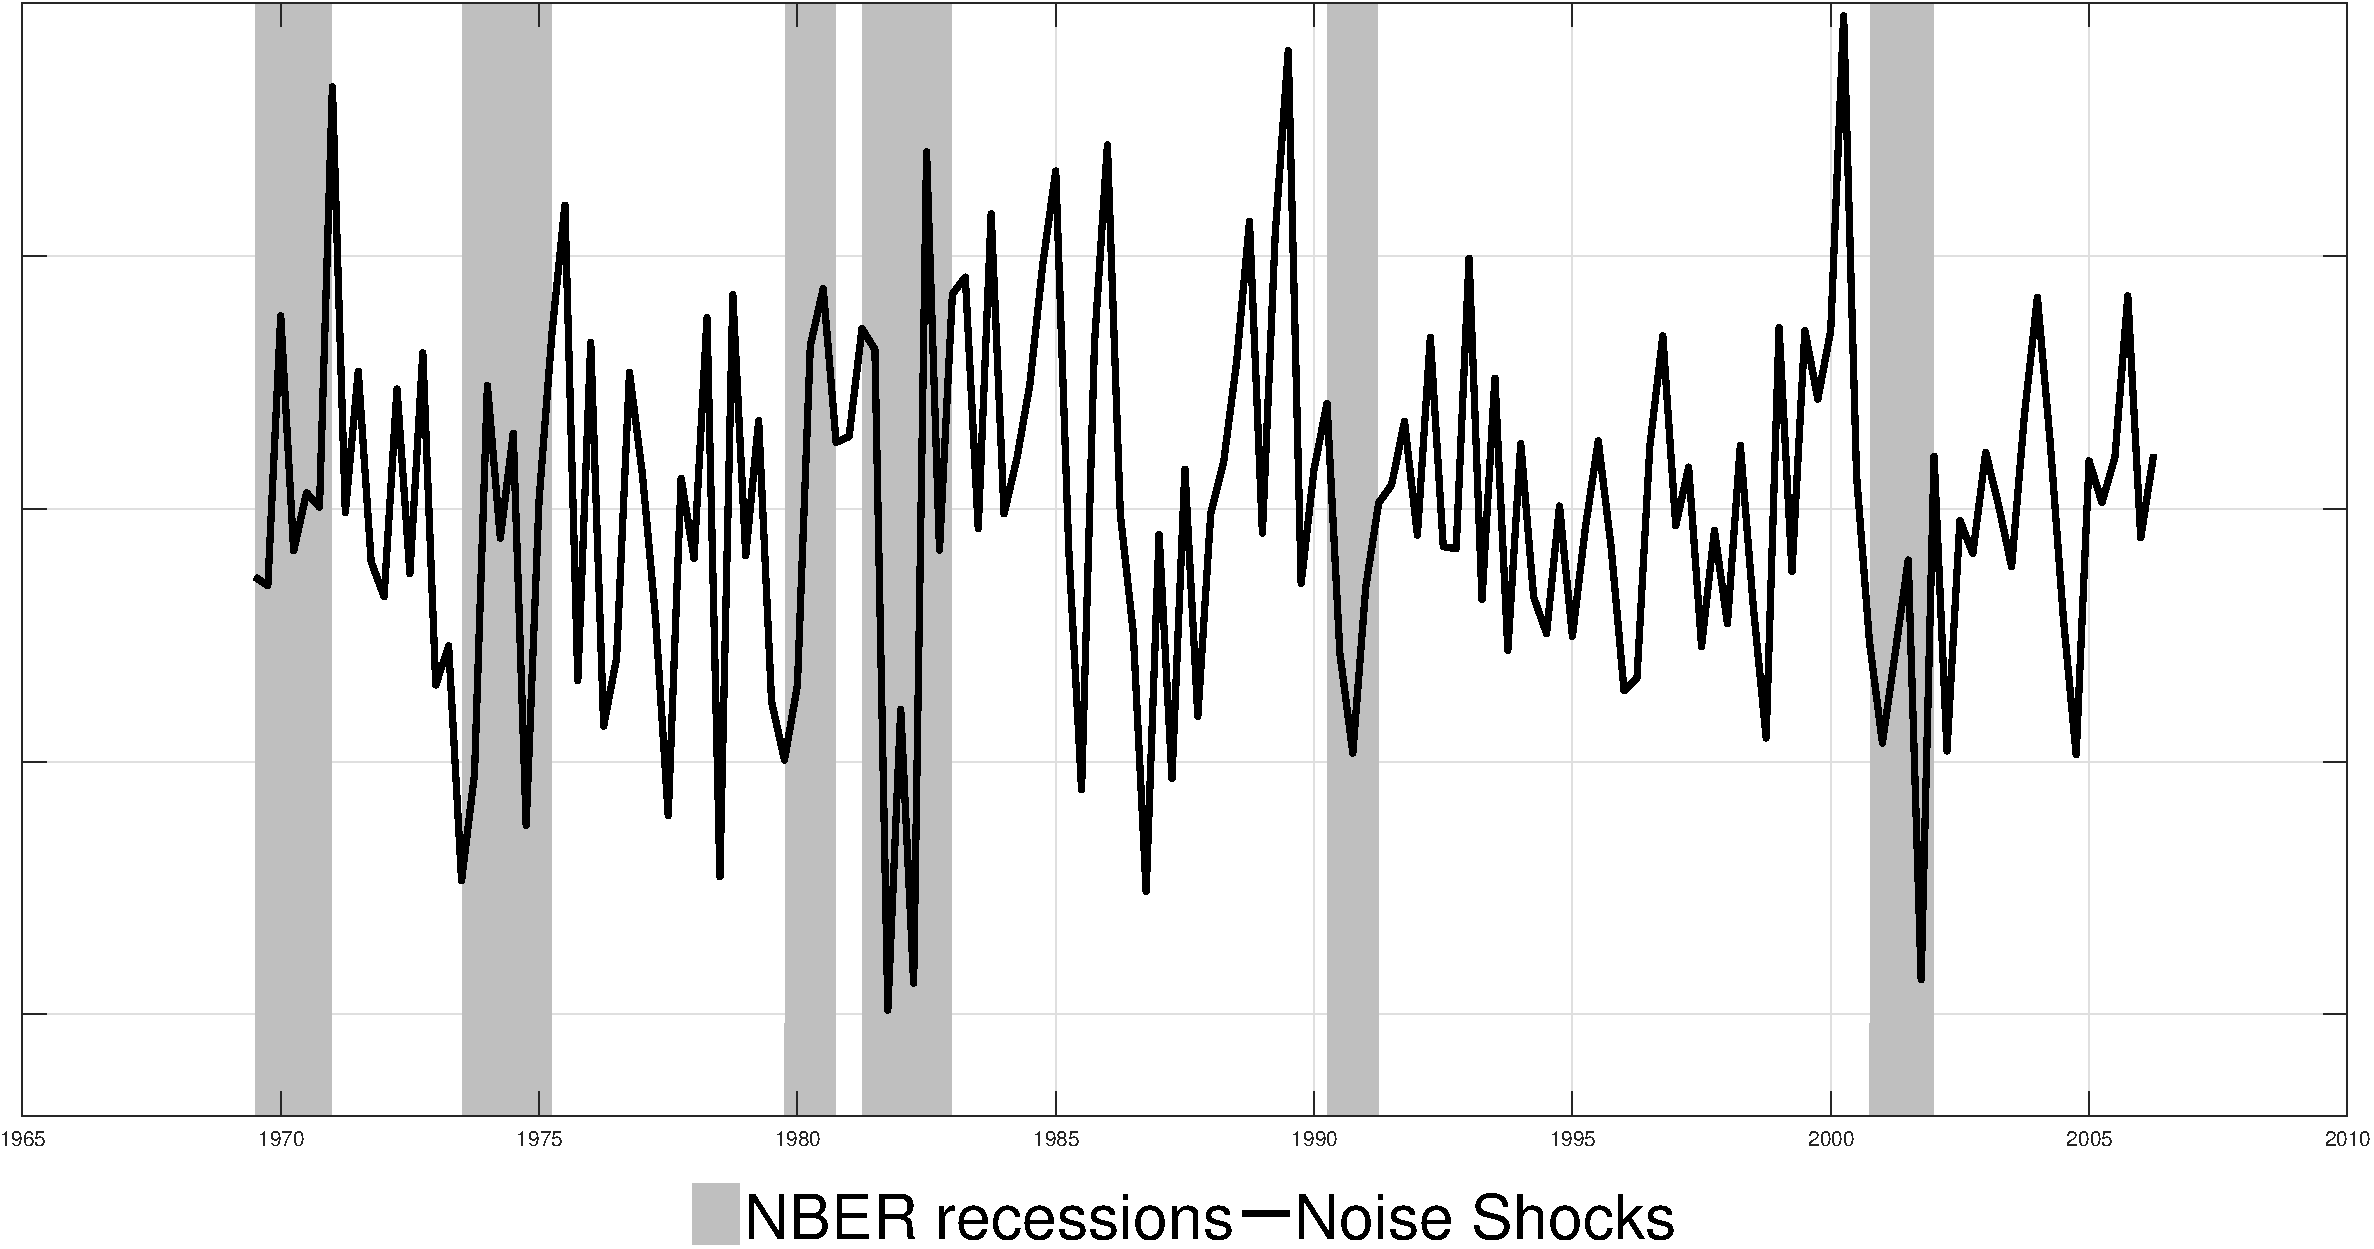
\includegraphics[scale = 0.27]{\ourFigPath Figures/Noise_Shocks_SPF_GDPgrowth_revisions}
\end{center}



}


\frame{\frametitle{Local Projection using Smooth Transition}
	
	\begin{center}
		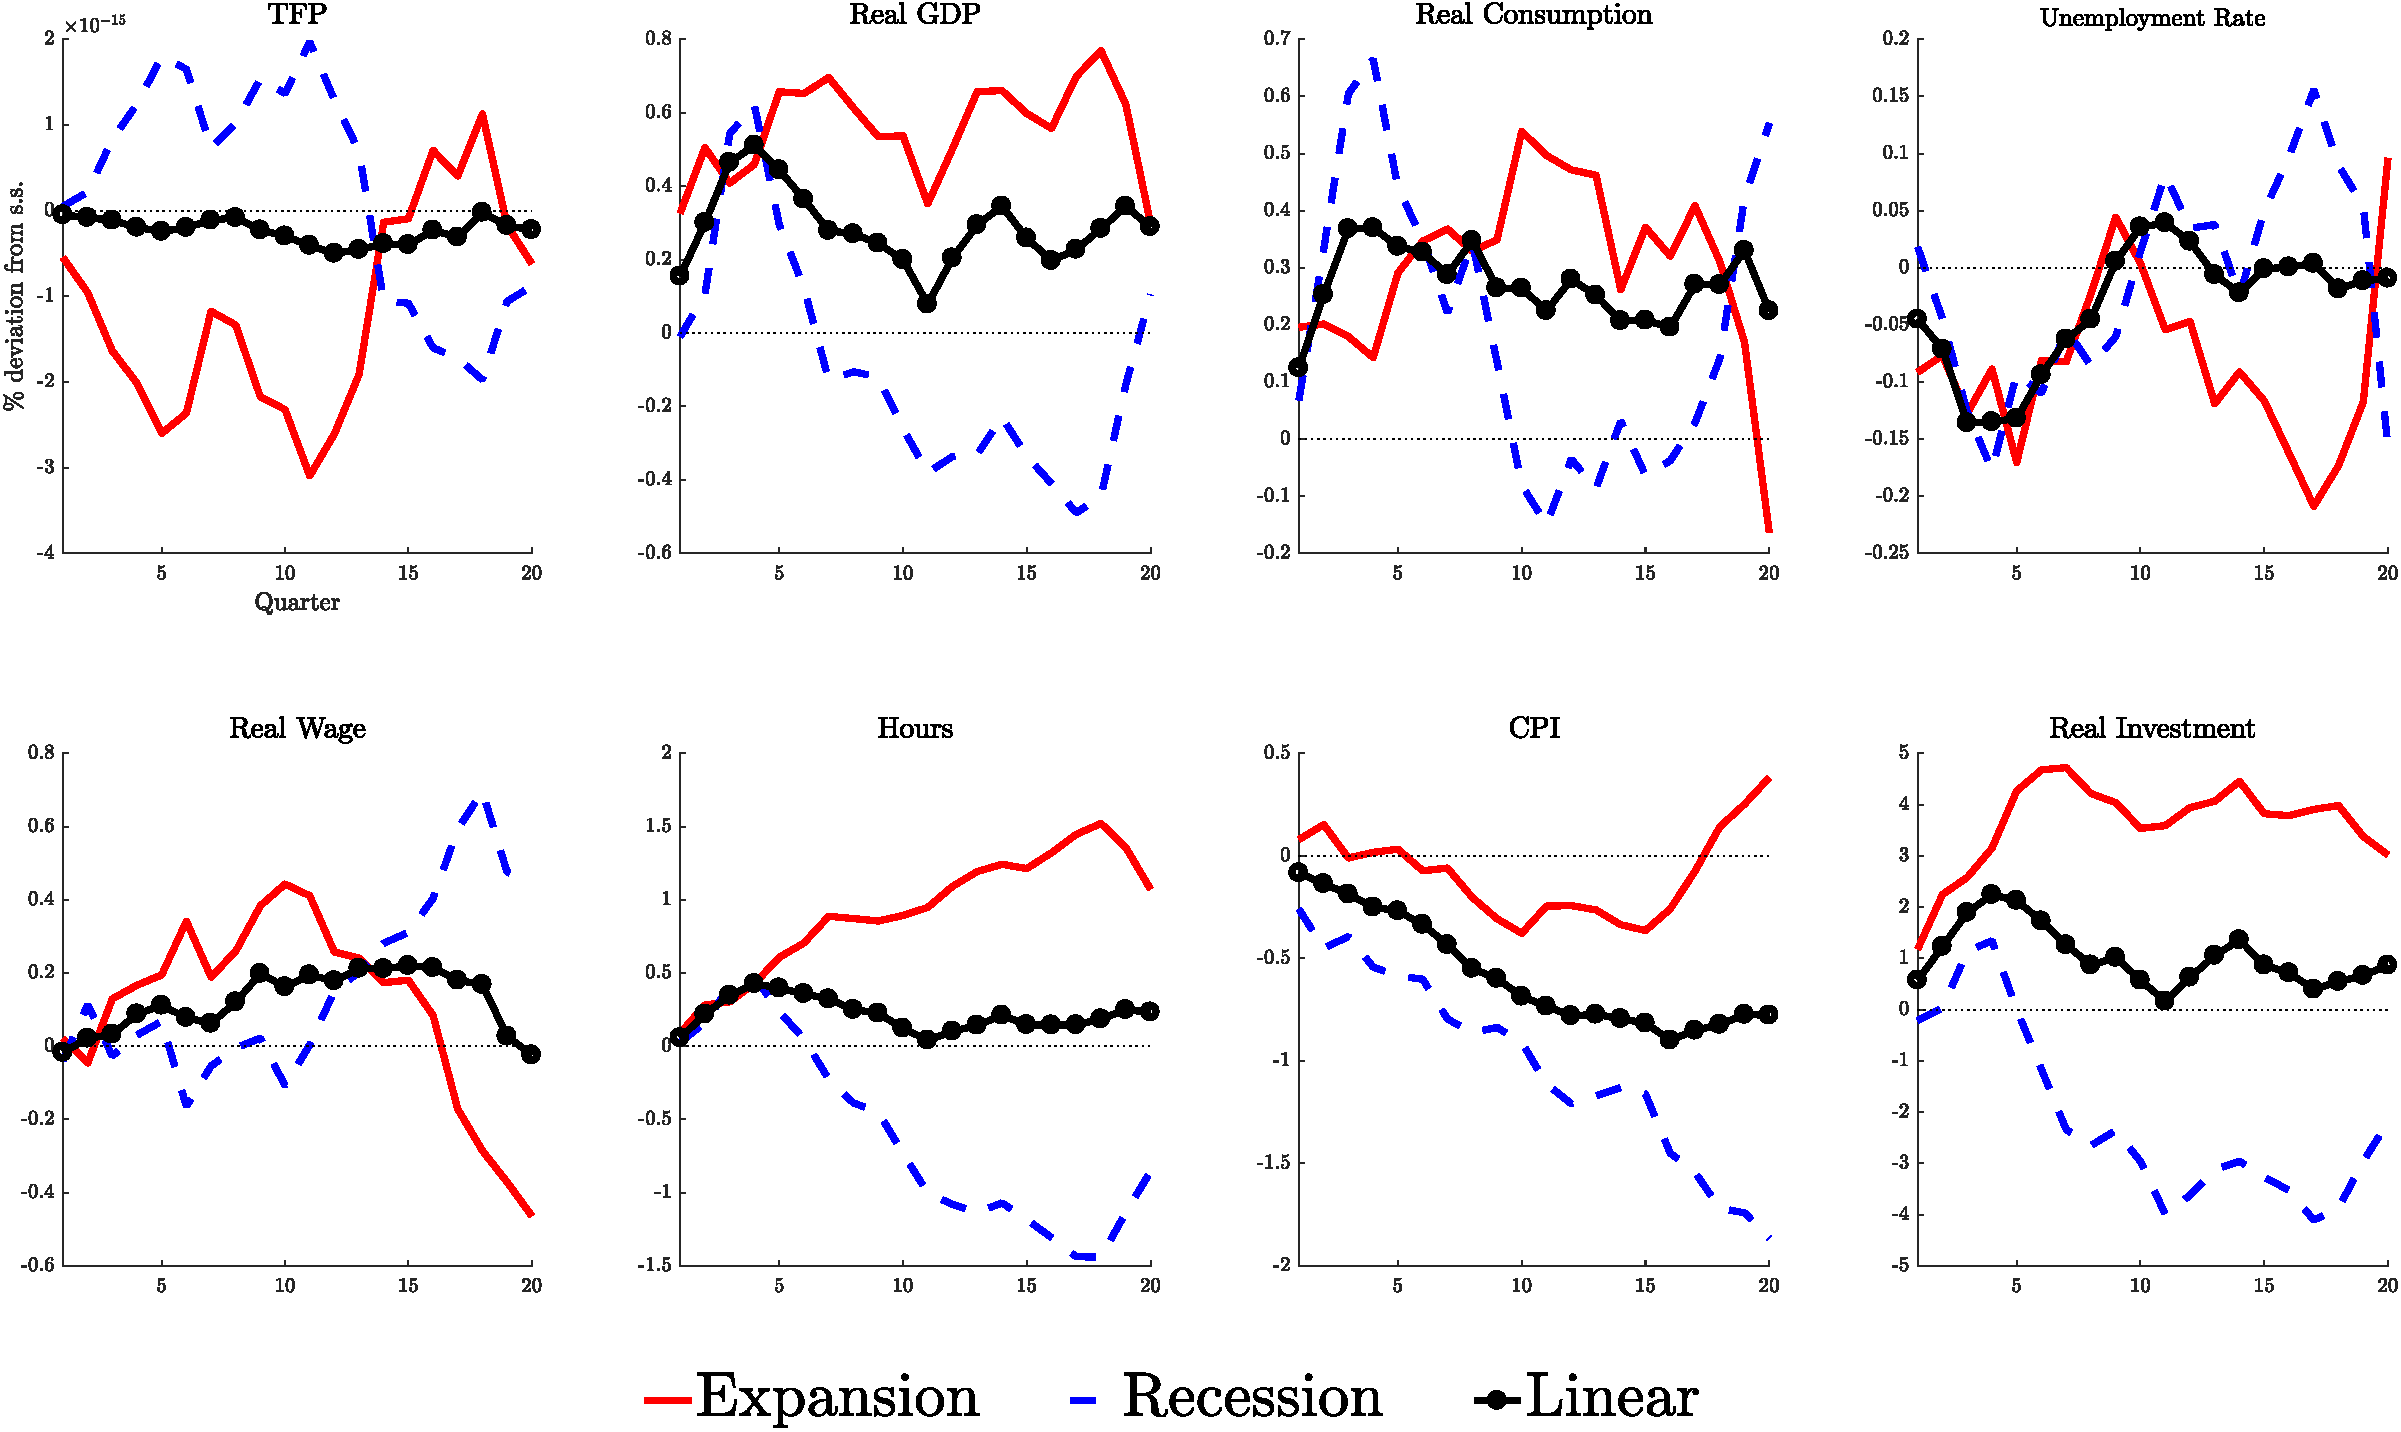
\includegraphics[scale = 0.27]{\ourFigPath Figures/STLP_IRFs_Noise_Shocks_SPF_GDPgrowth_revisions}
	\end{center}
	
	
	
}


\frame{\frametitle{Main Issues}
	
\begin{enumerate}
	\item SPF information set may be different to the one of economic agents.
	
	\
	
	\item Forecast horizon of SPF may be to short to properly capture future beliefs.
	
	\
	
	\item Do we need to treat for possible trend in the data? 
	
	\
	
	\item Need to set up a reliable procedure for the confidence intervals.
	
	\
	
	
	\item Need to allow for endogenous feedbacks of noise on $\eta_t$ in the local projection.
	\end{enumerate}
	
	
	
}









\begin{frame}[label=Details]
\frametitle{Details on $\eta_t$ and STPL procedure}

$\eta_t$ is defined as the seven-quarter moving average of the output growth rate. 
\begin{itemize}
	\item Notice that we can easily consider dynamic feedbacks from noise to the state of the regime.
\end{itemize}


\

\


Following Auerbach and Gorodnichenko (2012) we calibrate $\gamma$ to $1.5$ for now.\begin{itemize}
	\item Granger and Teravista (1993) suggest robustness checks procedure for $\gamma$.
\end{itemize}

\

\



\hyperlink{STLP}{\beamerbutton{Return}}

\end{frame}
\end{document}